\documentclass[12pt]{csethesis}
\usepackage[english]{babel}
\usepackage{amsmath}        % Extra math definitions
\usepackage{graphics}       % PostScript figures
\usepackage{setspace}       % 1.5 spacing
\usepackage{multicol}
\usepackage{bigints}
\usepackage{amssymb}
\usepackage{graphicx}
\usepackage{footnote}
\usepackage{lscape}
\usepackage{color}
\usepackage{array}
\usepackage{multirow}
\usepackage{sidecap}
\usepackage[table]{xcolor}
\usepackage{colortbl}
\usepackage{sidecap}
\usepackage{longtable}
\usepackage{wrapfig}
%\usepackage{hyperref}
\newtheorem{lemma}{Lemma}[chapter]
\makeatletter
\@addtoreset{lemma}{chapter}
\makeatother
\newtheorem{theorem}{Theorem}[chapter]
\makeatletter
\@addtoreset{theorem}{chapter}
\makeatother

\usepackage[left=1.5in,right=1in,top=1in,bottom=1in]{geometry}
%\usepackage[top=1cm,left=1cm,right=1cm,bottom=1cm]{geometry}
\usepackage{emptypage}
\usepackage{lipsum}
\usepackage{fancyhdr}
%\fancyfoot{}
%\fancyfoot{\thepage}
\fancyhead[RO,LE]{}
\fancyhead[RE]{\ifnum\value{chapter}>0 \bfseries{\nouppercase{\rightorleftmark}} \else \bfseries{\leftmark} \fi}
\fancyhead[LO]{\ifnum\value{chapter}>0 \bfseries{\nouppercase{\rightorleftmark}}  \else \bfseries{\leftmark} \fi}
%\fancyhead[LO]{ \bfseries\slshape\nouppercase{\rightorleftmark}}
\makeatletter
\newcommand{\rightorleftmark}{%
  \begingroup\protected@edef\x{\rightmark}%
  \ifx\x\@empty
    \endgroup\slshape\nouppercase{\leftmark}
  \else
    \endgroup\rightmark
  \fi}
\makeatother

\newtheorem{example}{Example}
\phdtitle = {Deep Learning Models for Handwritten English Character Recognition: Dataset Preparation and Performance Analysis}
\name = {Anmol Kulshreshtha}
\rollno = {21075011}
\guide = {Dr. Hariprabhat Gupta }

\begin{document}
\pagenumbering{roman}
\begin{titlepage}
% \textheight 15.5in \textwidth 12.5in {\raggedright \huge\bf \the\phdtitle}\\[70ex]
% \begin{flushright}
% \hspace{8cm}{\LARGE \bf \the\name}\\  [1ex] 
% \end{flushright}
%\pagebreak
\thispagestyle{empty}
\mbox{}
%\pagebreak
\begin{center}
\textheight 15.5in \textwidth 12.5in {\LARGE\bf  \the\phdtitle}\\[9ex]
\emph{Report submitted in fulfillment of the requirements\\
for the Exploratory Project of\\
[2ex]\large \bf Second Year B.Tech.
}\\
[2ex] \emph{by} \\[2ex]
{\large\sf \bf \the\name}\\ [7ex] 
   %          \the\rollno\\[6ex]
\emph{Under the guidance of}\\[1ex]
{\large \sf \bf \the\guide} \\[7ex]

\vspace{.05in}
\begin{center}
 
\includegraphics[scale=.7,keepaspectratio=true]{./logo.jpeg}
 % iitglogo.eps: 0x0 pixel, 300dpi, 0.00x0.00 cm, bb=
\end{center}
% 

%{\sl \bf{to the}} \\[1ex]
\vspace{1cm}
{\small  \bf Department of Computer Science and Engineering}  \\[1ex]
{\small \bf{INDIAN INSTITUTE OF TECHNOLOGY (BHU) VARANASI \\
Varanasi 221005, India\\
  May 2017}}

\end{center}
\end{titlepage}

\newpage
\thispagestyle{empty}
\mbox{}
%\onehalfspacing
\doublespacing
\chapter*{ }
\label{dedication}
\thispagestyle{empty}
\begin{center}
% \large\bf \lq\lq{}Om Vang Me Manasi Pratisthita\rq\rq{}\\
% \sl \lq\lq{}May my mind be stable in my speech, May Atman manifest  \\
% \sl unto me and reveal unto me the Highest Knowledge\rq\rq{}\\
% \bf-Aitareya Upanishad\\[18ex]
%\large\bf  In Memory of\\
%\large\bf  Dadu, Thakurda and Thakuma\\[18ex]
\Huge\bf  Dedicated to\\
\Huge \em My parents, teachers,.....\\[20ex]
\end{center}


\raggedbottom
\chapter*{\centering \underline{Declaration}}
\thispagestyle{empty}
I certify that
\begin{enumerate}
\item The work contained in this report is original and has been done by myself and the general supervision of my supervisor.
\item The work has not been submitted for any project.
\item Whenever I have used materials (data, theoretical analysis, results) from
other sources, I have given due credit to them by citing them in the text
of the thesis and giving their details in the references.
\item Whenever I have quoted written materials from other sources, I have put
them under quotation marks and given due credit to the sources by citing
them and giving required details in the references.
\end{enumerate} \vskip 10ex


\begin{table}\centering
\begin{tabular}{p{6cm}p{12cm}}
Place: IIT (BHU) Varanasi &\textbf{\the\name}\\
Date:  & B.Tech. or IDD Student\\
&Department of Computer Science and Engineering,\\
&Indian Institute of Technology (BHU) Varanasi,\\
&Varanasi, INDIA 221005.
\end{tabular}
\end{table}

\raggedbottom
%\doublespacing
%\pagenumbering{roman}
\chapter*{\centering \underline{Certificate}}
\thispagestyle{empty}
\vskip 2ex \emph{\quad This is to certify that the work contained
in this report entitled ``\textbf{\the\phdtitle}'' 
being submitted by \textbf{\the\name}
(\textbf{Roll No. \the\rollno}), carried out in the Department of
Computer Science and Engineering, Indian Institute of Technology (BHU) Varanasi, is a bona fide work of our supervision.} \vskip 15ex



\begin{table}\centering
\begin{tabular}{p{6cm}p{12cm}}
 & \textbf{Dr. Hariprabhat Gupta}\\
Place: IIT (BHU) Varanasi& Department of Computer Science and Engineering,\\
Date: &Indian Institute of Technology (BHU) Varanasi,\\
&Varanasi, INDIA 221005.
\end{tabular}
\end{table}
\chapter*{\centering Acknowledgments}
\thispagestyle{empty}
\quad I would like to express my sincere gratitude to Dr. Hariprabhat Gupta, Associate Professor, Department of Computer Science and Engineering, IIT (BHU) Varanasi for hir valuable insights into this project.
\\ \vskip 2ex
\noindent Place: IIT (BHU) Varanasi\\
Date: 20/4/2023 		\hskip 	45ex					{\textbf{\the\name}}
\newpage
\chapter*{\centering Abstract}
{

 In this project, we investigate the performance of various deep learning models for handwritten English character recognition. Specifically, we explore convolutional neural network (CNN), CNN with gated recurrent units (GRU), CNN with long short-term memory (LSTM), and LSTM models for this task. We also develop and utilize a dataset preparation pipeline to preprocess and augment the available data to improve model performance. Through comprehensive experimentation and performance analysis, we demonstrate the effectiveness of these models for handwritten English character recognition, with the CNN+LSTM model achieving the highest accuracy of all the models tested. Our work contributes to the field of handwriting recognition and provides valuable insights into the strengths and weaknesses of different deep learning models for this task.

The task of handwritten English character recognition has various practical applications, including but not limited to OCR (optical character recognition), document digitization, and text recognition for mobile devices. Our work on developing and analyzing deep learning models for this task is highly relevant and useful in these domains.

Furthermore, our dataset preparation pipeline can be used as a blueprint for preparing and augmenting datasets for other tasks in computer vision and deep learning. This can save significant time and effort in dataset preparation, especially for tasks involving limited amounts of data.



}

 

\pagestyle{fancy}
\tableofcontents
\clearpage
\addcontentsline{toc}{chapter}{\listfigurename}
\listoffigures
%\newpage
\thispagestyle{empty}
\mbox{}
%\clearpage
\addcontentsline{toc}{chapter}{\listtablename}
\listoftables
\addcontentsline{toc}{chapter}{List of Symbols}



 

\pagenumbering{arabic}
\def\headrulehook{\color{black}}      
%========== Chapters

\chapter{Introduction}\label{chap1}

\section{Overview}
Deep learning has revolutionized the field of computer vision, and character recognition is one of its most important applications. In this project, we focus on developing and analyzing deep learning models for handwritten English character recognition. Our dataset consists of preprocessed images of handwritten characters, which we use to train and test our models.

We explore the effectiveness of three different models - CNN, CNN with GRU, and CNN with LSTM - and evaluate their performance through comprehensive experimentation and analysis. Our experiments include comparing the accuracy and speed of the different models, as well as evaluating their robustness to noise and other image distortions.

Overall, our work has important practical implications for fields such as OCR, document digitization, and mobile device technology, where accurate and efficient character recognition is crucial. By leveraging the power of deep learning models, we have demonstrated the potential for achieving high accuracy in handwritten English character recognition, paving the way for more efficient and accurate processing of handwritten documents and text recognition on mobile devices.

we also optimize and fine-tune these models. We used a combination of different neural network architectures, including convolutional neural networks (CNN), long short-term memory (LSTM) networks, and gated recurrent units (GRU), to achieve the best results.

We also implemented various hyperparameter tuning techniques to optimize the performance of our models. This involved adjusting the learning rate, batch size, number of epochs, and other parameters to achieve the highest accuracy and efficiency.

To help visualize and analyze the results of our experiments, we used various types of graphs and charts, such as accuracy vs. epoch plots, loss vs. epoch plots, and confusion matrices. These graphs allowed us to identify areas where our models were performing well, as well as areas where they needed improvement.

\section{Motivation of the Research Work}\label{sec1.1}
The motivation behind my research work was to explore the field of deep learning and its applications in character recognition. I was particularly interested in the challenges posed by handwritten character recognition, where the variability in handwriting style and quality can make recognition a difficult task. I wanted to explore the effectiveness of deep learning models in accurately recognizing handwritten English characters and to compare the performance of different architectures.

Furthermore, I was motivated to take on the challenge of hyperparameter tuning to obtain the best possible performance from these models. I used various techniques such as grid search and random search to explore the hyperparameter space of each model, and plotted graphs to visualize the results and obtain insights into the behavior of the models. This required a lot of hard work and dedication, as it involved running multiple experiments and analyzing the results to fine-tune the models for optimal performance.


\chapter{Project Work}\label{final}

\textbf{\large Deep Learning Models for Handwritten
English Character Recognition:}

\\This section describes the startegy used for implementing character recognition from a given database. Before further proceeding, you are required
to know basic terminologies and definitions related to image database[3].\\\\
\textbf{Problem statement:} Given a dataset of hand-written English characters, the objective of this project is to implement hand-written character recognition using deep learning models. The goal is to explore various deep learning models and optimize their performance by tuning hyperparameters.\\\\

Research project involves implementing hand-written character recognition using a dataset of hand-written English characters. The project includes exploring different deep learning models and optimizing their performance by tuning various hyperparameters and plotting results of accuracy and loss in graphs.


To begin with,preprocessed the images using OpenCV, which likely involved converting the images to a format suitable for deep learning, such as resizing, normalization, and converting to grayscale.

Trained several deep learning models on the preprocessed dataset, starting with a convolutional neural network (CNN) which is commonly used for image classification tasks. This likely involved setting up the architecture of the CNN, including the number and type of layers, the activation functions, and other hyperparameters such as learning rate and batch size.

After training the CNN, proceeded to explore other deep learning models, such as an LSTM (long short-term memory) model combined with a CNN, followed by an RNN (recurrent neural network) and a GRU (gated recurrent unit) combined with a CNN. These models are commonly used for sequence prediction tasks and can be effective for handwriting recognition tasks.

Tuned various hyperparameters to optimize the model's performance, such as the number of layers, the number of neurons in each layer, the learning rate, the batch size, and others.

Finally,plotted the results of the accuracy and loss for each model, likely using graphs to visualize the performance of each model over time. This allowed you to compare the performance of each model and determine which one was most effective for your task.

Overall, project involved a thorough exploration of various deep learning models for hand-written character recognition, and a detailed analysis of their performance using hyperparameter tuning and visualization techniques.
 


\chapter{Conclusions and Discussion}\label{final}
 The present study involved exploring several deep learning models for handwritten character recognition using a dataset of hand-written characters in the form of images. The models used for this purpose included LSTM+CNN, CNN, and CNN+GRU, which were trained by hyper-tuning their parameters.
 
 Initially, a CNN model was trained on 26 small and 26 capital letters, achieving an accuracy of 98 percent for capital letters and 97 percent for small letters. This outcome demonstrated the ability of the CNN model to accurately recognize handwritten characters.

Subsequently, the CNN model was trained on all 52 classes, achieving an accuracy of 97.01 percent. This result indicates that the CNN model is capable of recognizing a broader range of handwritten characters with high precision.

The CNN+GRU model was then trained, and an accuracy of 97.61 percent was achieved. This outcome suggests that the addition of a GRU layer can potentially enhance the model's performance.

Finally, the LSTM+CNN model was trained and achieved an accuracy of 97.64 percent. This outcome represents the highest accuracy among all models tested and suggests that the incorporation of a recurrent layer, such as LSTM, can enable better capturing of long-term dependencies in the data.

In conclusion, the present study demonstrated the successful implementation of various deep learning models for handwritten character recognition using a dataset of hand-written characters in image format. The obtained results indicate that the incorporation of recurrent layers, such as LSTM and GRU, can enhance the performance of CNN models for this purpose.

\begin{figure}[htp]
    \centering
    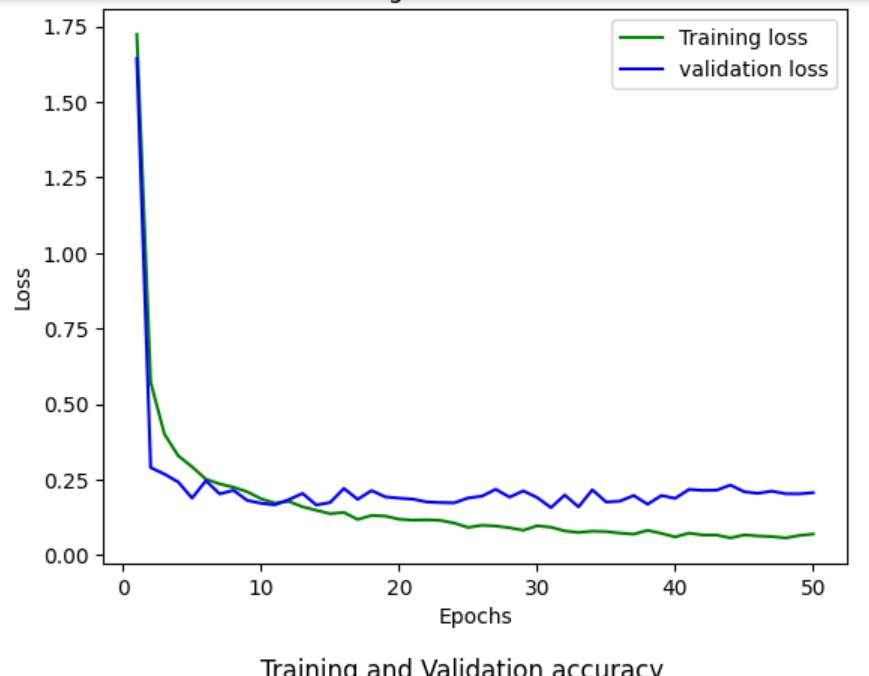
\includegraphics[width=8cm]{report/image1.png}
    \caption{The training and validation loss obtained from running a CNN model for 50 epochs}
    \label{fig:galaxy}
\end{figure}

\begin{figure}[htp]
    \centering
    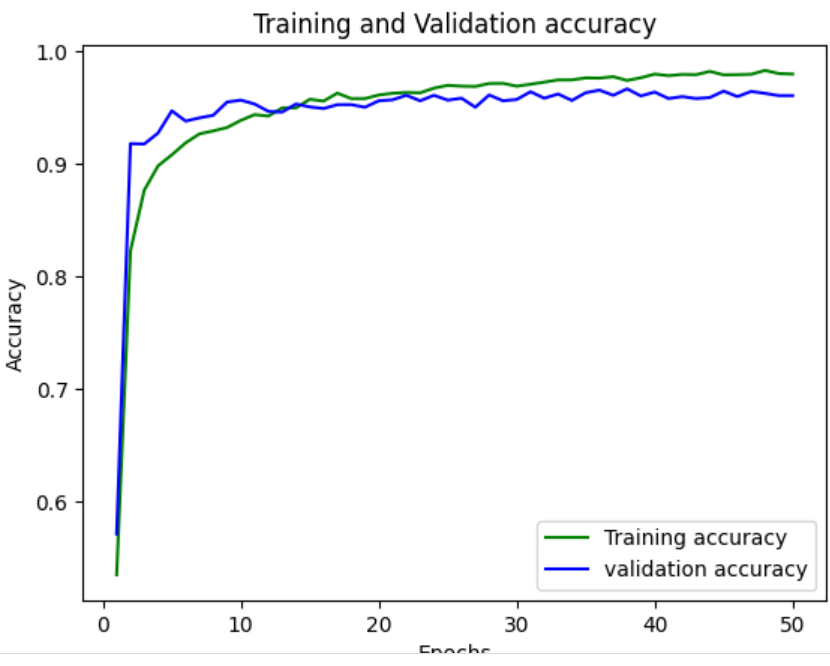
\includegraphics[width=8cm]{report/image2.png}
    \caption{The training and validation accuracy obtained from running a CNN model for 50 epochs}
    \label{fig:galaxy}
\end{figure}


\begin{center}
\begin{tabular}{||c c||} 
\hline
 Model & Accuarcy \\ [0.5ex] 
 \hline\hline
 CNN &  97.01  \\ 
 \hline
 ConvoGRU & 97.61 \\
 \hline
 CNN+LSTM & 97.64 \\ [1ex] 
\hline
\end{tabular}
\end{center}
\begin{center}
\caption{Table showing the accuracy of three different models }
\end{center}
\chapter{Bibliography}\label{final}

[$1$]  LeCun, Y., Bengio, Y., & Hinton, G. (2015). Deep learning. Nature, 521(7553), 436-444.\\\
[$2$]  Simonyan, K., & Zisserman, A. (2014). Very deep convolutional networks for large-scale image recognition. arXiv preprint arXiv:1409.1556.\\\
[$3$]  Goodfellow, I., Bengio, Y., & Courville, A. (2016). Deep learning (Vol. 1). MIT press.\\\
[$4$]  Krizhevsky, A., Sutskever, I., & Hinton, G. E. (2012). Imagenet classification with deep convolutional neural networks. In Advances in neural information processing systems (pp. 1097-1105).\\\
[$5$]  Abadi, M., Barham, P., Chen, J., Chen, Z., Davis, A., Dean, J., ... & Zheng, X. (2016). TensorFlow: A system for large-scale machine learning. In 12th USENIX Symposium on Operating Systems Design and Implementation (OSDI 16) (pp. 265-283).\\\
[$6$]  Chollet, F. (2017). Deep learning with Python. Manning Publications.\\\
[$7$] Graves, A., Mohamed, A. R., & Hinton, G. (2013). Speech recognition with deep recurrent neural networks. In IEEE international conference on acoustics, speech and signal processing (pp. 6645-6649).


\bibliographystyle{IEEEtran}
\bibliography{report}
\end{document}
